\chapter{Literature Review}
\section{Cybersecurity}
\subsection{Memory vulnerabilites and safety}
\paragraph{}Memory unsafety is one of the main sources of vulnerabilite is in software new and old. The USA Biden-Haris administration have pushed for these issues to be solved through the use of memory safe programming languages, and hardware mitigations \autocite{noauthor_fact_2024}.

\paragraph{}It was explained in \cite{aleph_one_smashing_1996} that many C programs could be exploited using a buffer overflow vulnerability. This is a type of memory vulnerability where the length of an input it not checked against the length of the memory buffer being used to store the memory. If the data is therefore longer than the buffer can store this leads to memory inside the program being overwritten. The term "smashing the stack" comes from using this behavior to overwrite the programs stack; which is possible if the stack is stored in higher memory addressed than the buffer being targeted. Since the stack contains return addresses and the contents of variables this attack can be used to maniuplate the behavior and control flow of the program. In systems without any protection this can even lead to the attacker inserting their own executable machine code into the programs memory space then ordering the program to jump to it by manipulating return addresses inside the stack.

\paragraph{}Multiple strategies have been used to detect, mitigate, or prevent memory vulnerabilities. These include \acrshort{aslr}, \acrshort{dep}, fuzzing, stack protectors/canaries, dynamic analysis focusing on memory allocation, and memory safe languages.

\paragraph{}\acrfull{aslr} works by randomly arranging the location of the different memory segments in an application such as the stack, heap, libraries, and so on. This means each time a program runs it will have a different layout in memory making targeting specific memory regions inside the program using a buffer exploit to be more difficult, therefore decreasing the explitability of buffer exploits \autocite{syedishrarali_aslr_2024}. Unfortunately, this is not a perfect defense, as \acrshort{aslr} does not actually stop the exploit from overwriting memory, so while it can render an attack unsuccessful in gaining access, it can still cause the program to crash or behave unexpectedly. There are a variety of techniques that can be used to bypass \acrshort{aslr} such as \acrfull{rop}, Ret2libc, heap spaying, information leakage, and brute force attacks. \autocite{gallucci_aslr_2024}. This means that ASLR alone is not sufficient to prevent attacks.

\paragraph{}Fuzzing is a technique that can be used to find vulnerabilities in software. It is a technique that involves creating a set of input called fuzz and feeding it to a program. Unlike other analysis techniques, it can be used even without access to the program source code. The fuzz in question could come in different forms depending on the program being tested including network traffic, files, strings, or even executables. Ideally fuzzed inputs are not rejected immediately for data validation reasons as this allows for more testing and code coverage. This technique works not only for memory vulnerabilities, such as buffer overflows, but for other classes of vulnerability, such as cross-site scripting and denial of service vulnerabilities. OSS-Fuzz is a Google-designed fuzzing project that can Fuzz programs written in C, C++, Rust, Go, or Python using multiple fuzzing engines with automatic reporting of discovered vulnerabilities. Some fuzzers use knowledge of the application structure to target their testing data for the program, while others can operate on black-box programs and don't require any knowledge about program internals. \autocite{beaman_fuzzing_2022}

\paragraph{}Stack canaries/security cookies are a technique to detect a buffer overflow attack in progress so that the program being attacked can be terminated. It does this by placing extra data before or after key values in the stack such as return addresses. An attacker attempting to mess with the program could end up clobbering these values, thereby causing the attack to be detected and program terminated. There are several types of stack caneries including null canaries, terminator canareis, and random canaries. Random XOR canaries are the most secure as an attacker would have to guess or obtain the correct value to exploit the program. A program that has a memory leak may allow for obtaining the value of the canaries during execution and so allow the security mechanism to be bypassed. \autocite{michiel_lemmens_stack_2021}

\paragraph{}Memory safe languages are languages that in some way attempt to prevent memory vulnerabilities in new software created using them. According to \cite{rina_diane_caballar_move_2023} the majority of modern programming languages are already memory safe. Some recommended modern languages include Rust, Kotlin, and Swift.


\section{\acrlong{ai} and \acrlong{llm}}
Some LLMs that will be discussed in this section:

\begin{itemize}
\item{Gemma 3}
\item{DeepSeek R1}
\item{Mixtral}
\item{Qwen}
\end{itemize}

\paragraph{} The paper \textcite{deepseek-ai_deepseek-r1_2025} tells us about DeepSeek's R1-Zero and  R1 models. In particular it says that the models are based on the existing DeepSeek V3 MoE model, but have been further trained to allow for \acrfull{cot} reasoning similar to ChatGPT's O1. ChatGPT O1 is one of the first \acrshort{cot} models and is closed source. R1-Zero was created by applying reinforcement learning to the V3 model, which was successful in producing a model with \acrshort{cot} capabilities. It did however have problems such as language mixing. To deal with these issues another model was created, called R1. R1 used both reinforcement learning like R1-Zero, but also used supervised fine tuning with a small amount of cold-start data. This lead to a model without the issues seen in R1-Zero. The paper also covers a technique called distillation: this is where a larger model like R1 is used to train smaller models. In this case distillation was used to train multiple \acrshort{llama} and Qwen base models to have Chain of Thought capabilities. This technique was compared against doing reinforcement learning directly on the \acrshort{llama} and Qwen models to create Chain of Thought reasoning. It was found that the distillation technique resulted in more effective small models. Both the full model and the distilled models have been open-sourced.

\paragraph{}Qwen have a series of models they have released. One of these is a reasoning model called qwq. According to their benchmarks from \textcite{} it has performance comparable to the full 671 billion parameter DeepSeek R1 despite only being 32 billion parameters in size. It also compares favorably to OpenAI's o1-mini and the smaller distilled versions of DeepSeek R1. These benchmarks are shown in a copy of their graph in figure \ref{fig:qwq-performance}.

\begin{figure}
    \centering
    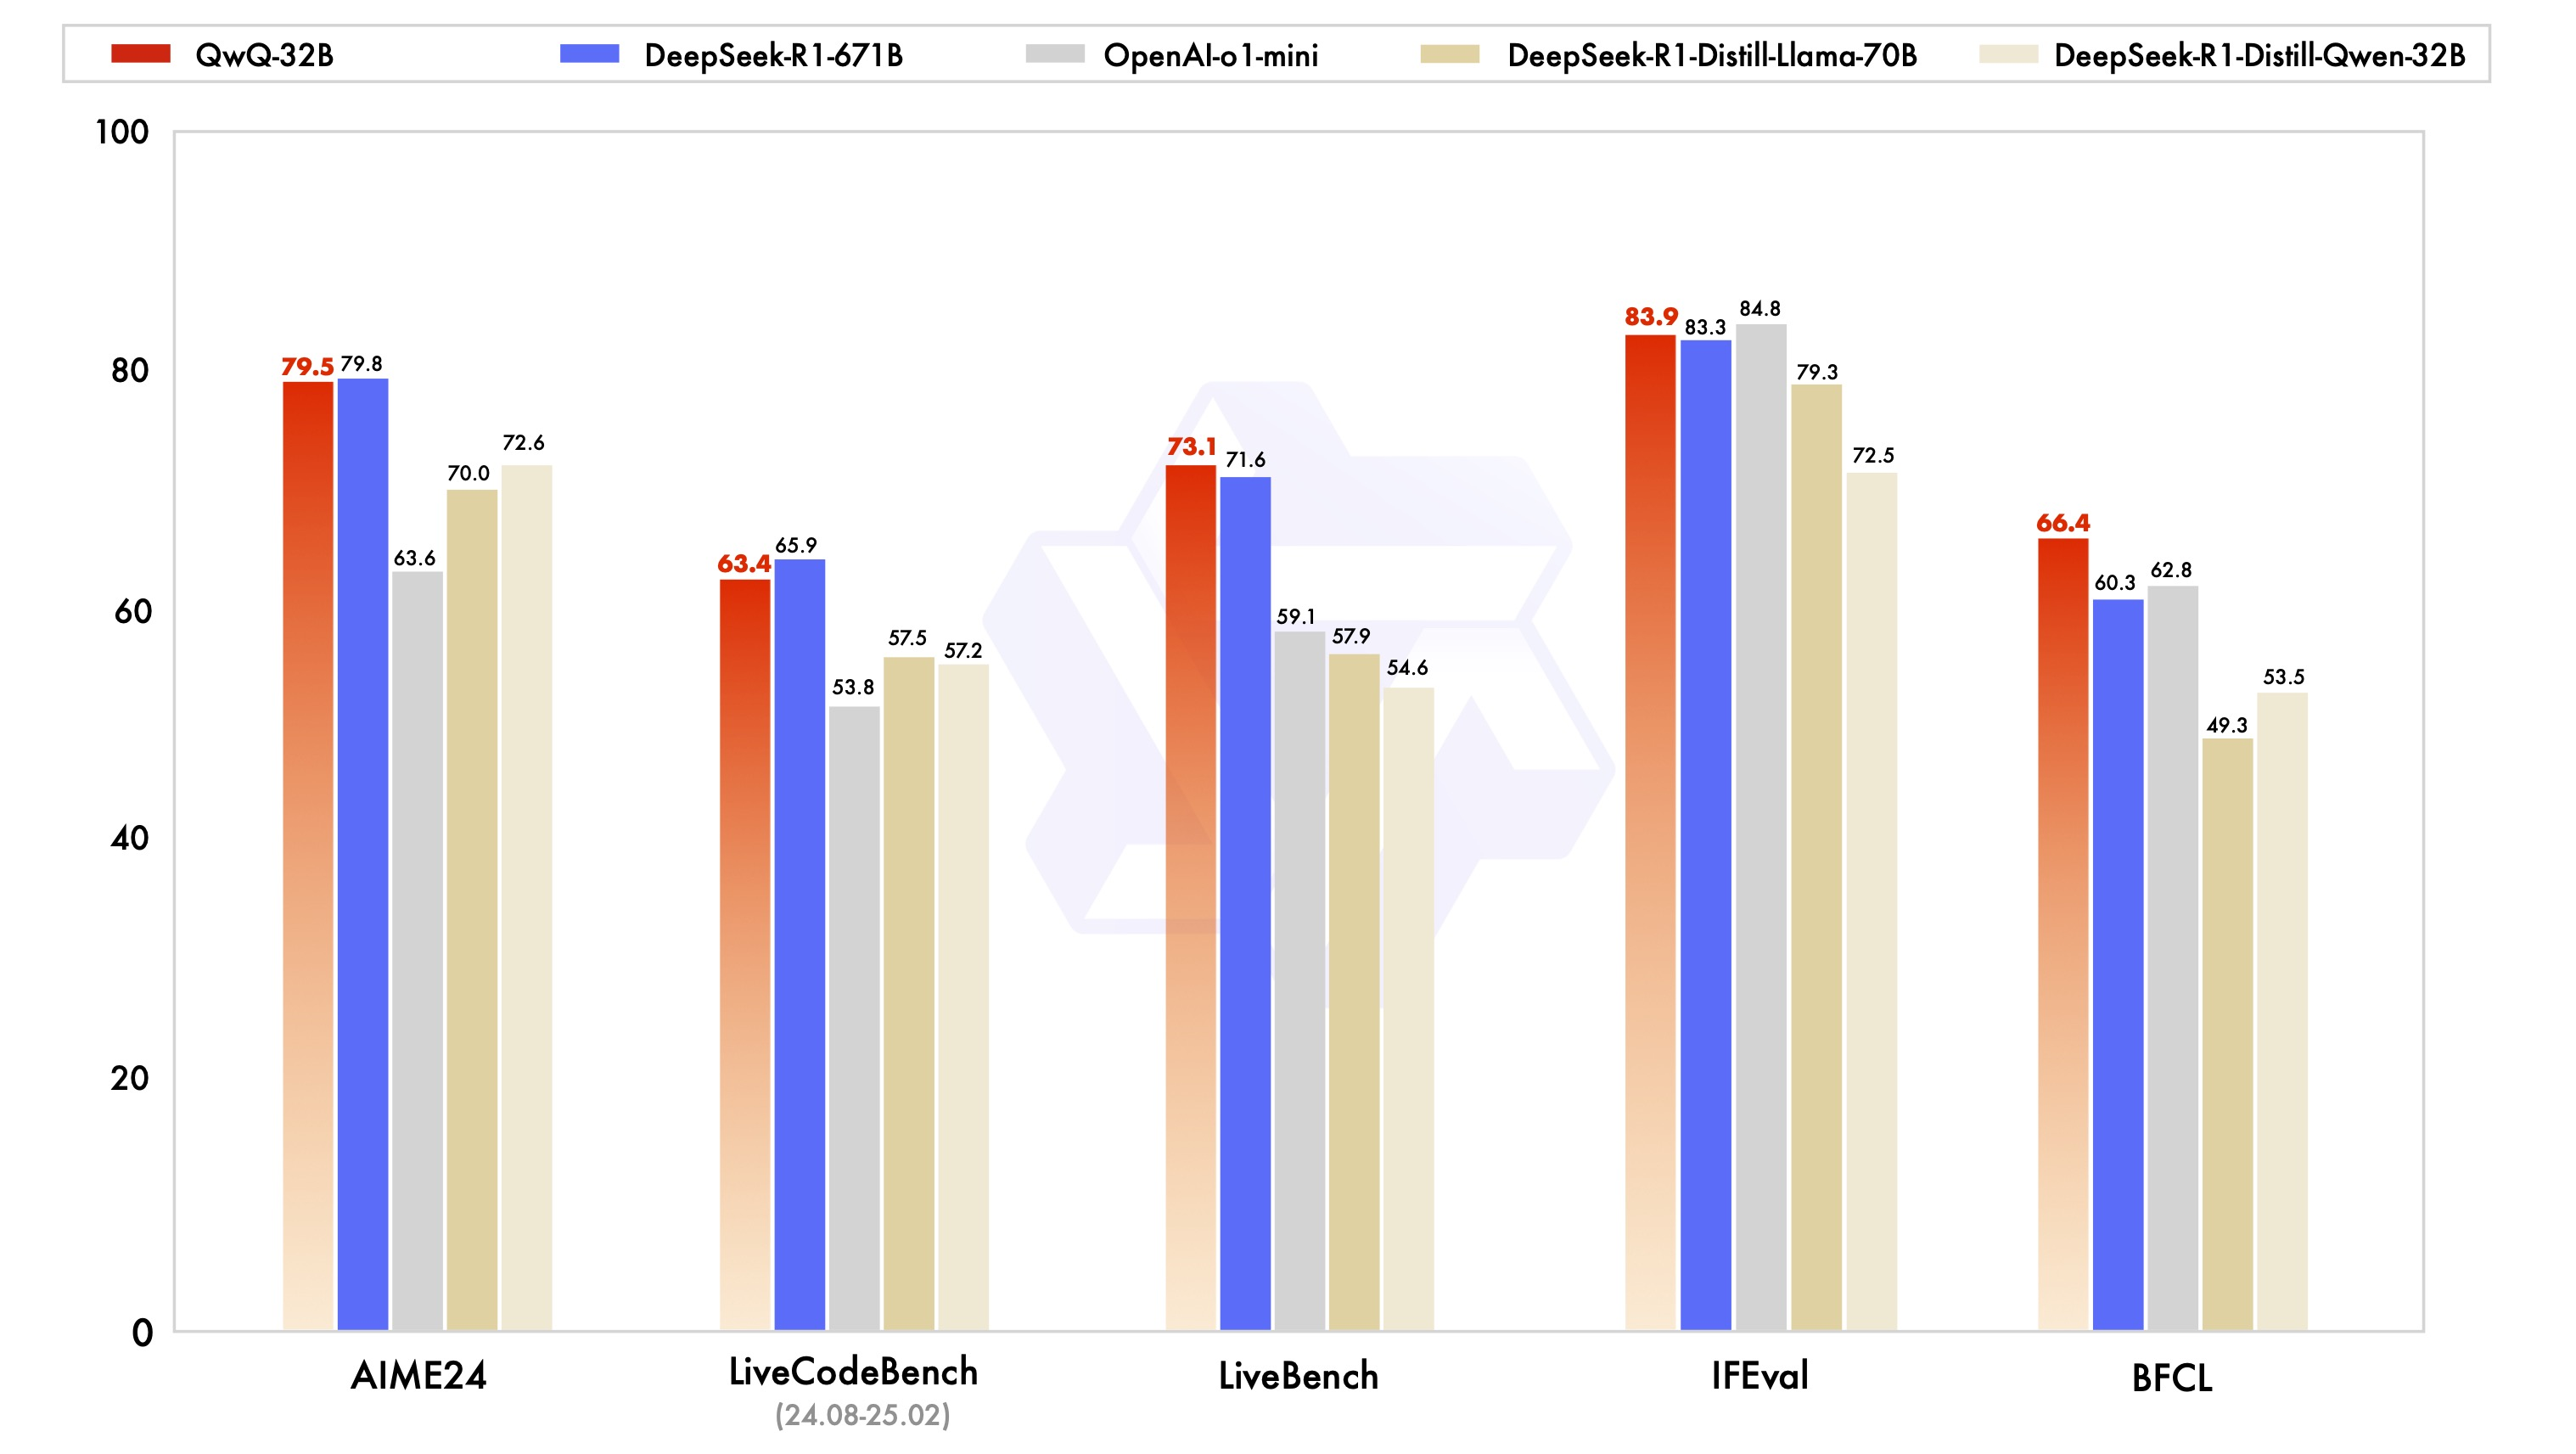
\includegraphics[width=1\linewidth]{figure/qwq-32b-final.jpg}
    \caption{QwQ performance in benchmarks}
    \label{fig:qwq-performance}
\end{figure}

\paragraph{}\autocite{chen_parallel_2025} is a paper exploring a new way of improving \acrshort{llm} performance through a new kind of scaling rule. Rather than using parameter scaling (making larger dense or MoE models), or inference time scaling (reasoning models), this instead uses one set of parameters being executed in parallel and the results combined together. By creating a model using this method, they were able to come up with something that requires a fraction of the memory than a similar performing dense model while having improved lantecy. Table \ref{tab:compare} is a copy of the table from this paper showing the advantages and disadvantages of different LLM scaling methods.



%Table from study
{
\begin{table}[t]
\caption{Copy of comparison table from \textcite{chen_parallel_2025}}
\centering
\resizebox{\linewidth}{!}{
\begin{tabular}{lllll}
\toprule
Method & Inference Time & Inference Space & Training Cost & Specialized Strategy \\
\midrule
Dense Scaling &  \emoji{figure/neutral_face} Moderate & \emoji{figure/rage} High & \emoji{figure/rage} Pre-training only & \emoji{figure/grin} No \\
MoE Scaling & \emoji{figure/grin} Low & \emoji{figure/rage} High & \emoji{figure/rage} Pre-training only & \emoji{figure/rage} \makecell[l]{Load balancing} \\
\makecell[l]{Inference-Time Scaling} & \emoji{figure/rage} High & \emoji{figure/neutral_face} Moderate & \emoji{figure/grin} \makecell[l]{Post-training} & \emoji{figure/rage} \makecell[l]{RL / reward data} \\
Parallel Scaling & \emoji{figure/neutral_face} Moderate & \emoji{figure/neutral_face} Moderate & \emoji{figure/grin} \makecell[l]{Pre- or Post-training} & \emoji{figure/grin} No \\
\bottomrule
\end{tabular}
}
\label{tab:compare}
\end{table}
}

\subsection{Image generation models}
\paragraph{}

\subsection{Fine Tuning models}

\subsection{\acrfull{rag}}
\acrshort{rag} is a technique that allows an LLM to access external data. This is done by having the LLM send the data to another model. This is converted to an embedding/vector. The embedding model uses this to search through a index of a knowledge base. This index also contains vectors that are compared against the vectors of the query. The retrieved information if then sent back to the LLM to generate a response. \acrshort{rag} could be used in a variety of applications including helping lawyers, doctors, and financial analysts with questions. \autocite{merritt_what_2025}.

\subsection{Agentic \acrshort{ai}}
\paragraph{}Agentic \acrshort{ai} is capable of goal-oriented, autonomous action and is adaptable. These \acrshort{ai}s are based on generative \acrshort{ai} such as LLMs. Unlike conventional LLMs they are not limited to the information they are trained on as they can do things such as independently gather new information. Like an LLM an agentic \acrshort{ai} can be interacted with through a natural language prompt, making them simpler to use than other software products. \autocite{noauthor_what_2025}.

\paragraph{}According to \textcite{pounds_what_2024} agentic \acrshort{ai} uses a four step process:
\begin{enumerate}
    \item Perceive
    \item Reason
    \item Act
    \item Learn
\end{enumerate}

\paragraph{}The last step called learn involves gathering data from the system in use, and using it to train future iterations of the model. This creates a feedback loop called the data flywheel.

\subsection{\acrshort{ai} in Scenario Generation}

\paragraph{}

\subsection{Character \acrshort{ai} and chatbots}